%% Regular, article-style document with 12pt font and A4 sized paper
\documentclass[12pt,a4paper,notitlepage]{article}

%% IEEE style alternative
%\documentclass[final]{IEEEtran}

%% UTF-8 support
\usepackage[utf8]{inputenc}

%% Basic packages for formulas, symbols, etc
\usepackage{amsmath}
\usepackage{amsfonts}
\usepackage{amssymb}
\usepackage{multirow}

%% Clean paragraph spacing
\usepackage{parskip}

% For page margins
\usepackage[left=2cm,right=2cm,top=2cm,bottom=2cm]{geometry}

%% Hyperlink support
\usepackage[colorlinks = true,
linkcolor = blue,
urlcolor  = blue,
citecolor = blue,
anchorcolor = blue]{hyperref}

%% Image support
\usepackage{graphicx}

%% For description sections (indentable lists)
\usepackage{enumitem}

%% Font improvements
\usepackage[T1]{fontenc}
\usepackage{lmodern}

%% Header and footer styles (page number centered at the bottom)
\usepackage{fancyhdr}
\usepackage{lastpage}

% Title text (not on separate page)
\usepackage{titling}

% Graphics
\usepackage{graphicx}
\graphicspath{ {../presentation/images/} }
\usepackage{float}
\usepackage{placeins}

% Title information
\pretitle{\begin{center}\Large\bfseries}
\posttitle{\par\end{center}\vskip 0.5em}
\preauthor{\begin{center}}
\postauthor{\end{center}}
\predate{\par\centering}
\postdate{\par}

\title{Effect of stroke width on semi-automatic image segmentation algorithms}
\author{Katrina Hoffert under supervision of Dr Mark Eramian}
\date{2016-2017}

% Page numbering
\pagenumbering{arabic}
\pagestyle{fancy}
\fancyhf{} %% Remove the default header/footer
\renewcommand{\headrulewidth}{0pt} %% Remove the header bar
\cfoot{\thepage} %% New footer content

\begin{document}

\maketitle
\thispagestyle{empty}

%% Abstract
\begin{abstract}
Semi-automatic image segmentation involves user interaction to some degree to assist in segmenting an image into multiple parts. Specifically, we looked at the category of algorithms that involve the user marking some areas as foreground and background. Past studies at the University of Saskatchewan had used user strokes or points that were always one pixel wide. This study looked at how the width of the stroke size influenced the results, with respect to accuracy (measured with the Dice similarity coefficient) and reproducibility (measured with the general Tanimoto coefficient).

All user strokes were dilated between 1-4 pixels and then used to segment the image. This was done with the Boykov max flow graph cut algorithm and also tested on the OneCut algorithm. We used images and user annotation data from two past studies, which both used images from the Berkeley Segmentation Dataset 500.

We found that dilating the strokes to have a radius of 4 pixels wide increased the mean DSC by between 0.010 to 0.065 and mean GTC increased between 0.061 and 0.069 (p < 0.01 for comparisons between non-dilated and 4 pixel dilation) with the primary segmentation algorithm. The result was also more significant when the user had more time to markup the images. This indicates that thicker strokes tend to get more accurate and more consistent results with thicker stroke values for our segmentation algorithm.

\end{abstract}

\section{Introduction}

\subsection{An intro to image segmentation}
The goal of image segmentation is to partition an image into distinct segments. Semi-automatic image segmentation utilizes some degree of user interaction to assist in this segmentation (but without making the user do all the work). Specifically, our study is concerned with the type of semi-automatic image segmentation that segments a foreground object from its background.

The method of user interactivity that this study looks at is where the user annotates what is foreground and what is background via applying points or strokes to an image. The segmentation program then takes in those user annotations (the ``label image'') and the image to be segmented and outputs a binary segmentation mask (which could be used to, say, separate the foreground and background).

Figure \ref{fig:example_combined} demonstrates the types of images involved in the process. At the top left we have the image we want to segment. The top right shows an example of user annotations (red = foreground, green = background). The bottom left shows the resulting segmentation and the bottom right shows the ground truth, which is the correct segmentation.

\begin{figure}[h]
	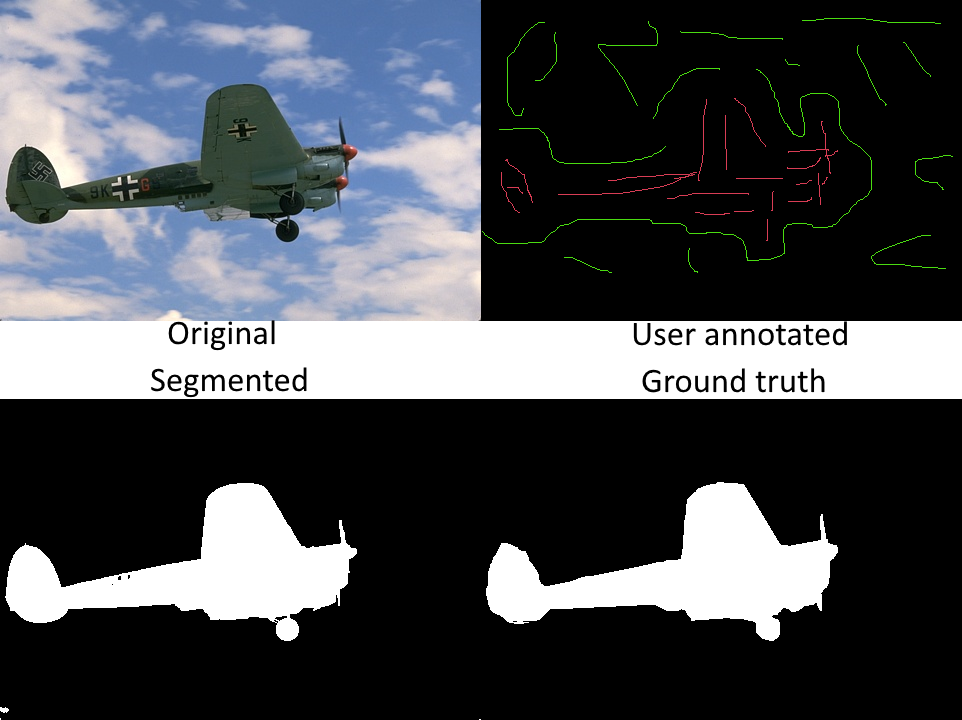
\includegraphics[width=\linewidth]{example_combined}
	\caption{The files involved in segmenting an image.}
	\label{fig:example_combined}
\end{figure}

\subsection{Problem}
The question that we're trying to solve is ``what is the impact of the width of these strokes?'' Or in other words, how much does the stroke width affect the quality of image segmentation? All the previous experiments in semi-automatic image segmentation conducted at the University of Saskatchewan had used 1 pixel wide strokes and points. There's the question of how different the segmentation result would be if the strokes were thicker (if at all).

Thicker strokes means that there's more annotations for the algorithm to use as ``seeds'' for segmenting and that any noise would have less of an impact. However, it's hard to say how much this could impact any given algorithm (and the results are surely algorithm dependent, as well). Thicker strokes can also mean that errors could be introduced due to the strokes now overlapping both the foreground and background. The impact of errors may vary with the algorithm, as well.

\subsection{Data sources}
This study uses two previous studies to provide user annotations that we can work on:

\begin{enumerate}
	\item In \textit{Analysis of User Input Methods For Semi-Automatic Segmentation} by Steven Rau \cite{rau}, the study contrasted the differences between user annotations that were strokes vs points.
	\item In \textit{Effects of Time Pressure on Semiautomatic Segmentation} by Yuanxia Li \cite{yuanxia}, the study contrasted the differences between 15, 25, and 40 second time limits for annotating each image.
\end{enumerate}

Both of these studies provide the needed format of having the forground and background marked by the user. They also do introduce some additional independent variables that we must treat separately (strokes versus points and 15s versus 25s versus 40s time pressures). All data in the study by Li used points.

All of the images in these studies comes from the Berkeley Segmentation Data Set and Benchmarks 500 \cite{bsds500} (BSDS500). Figure \ref{fig:bsds500_samples} provides examples of images that would be segmented. Note how some images are clearly easier to segment than others (eg, because the foreground and background have pronounced differences). The BSDS500 also provides us with the ground truth images that we need to analyze the segmentation results.

\begin{figure}[h]
	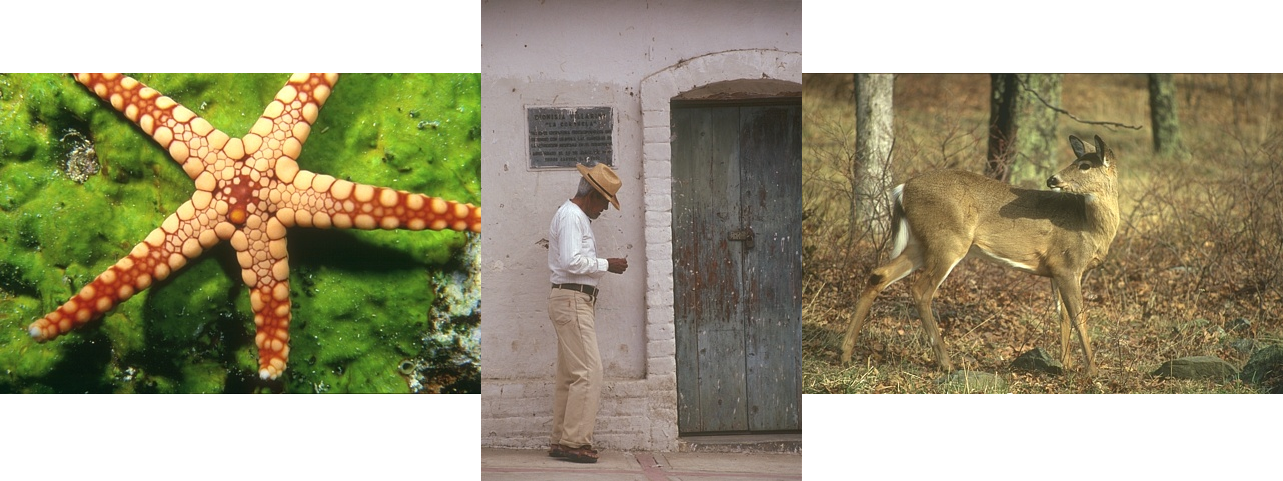
\includegraphics[width=\linewidth]{bsds500_samples}
	\caption{Example files from the BSDS500.}
	\label{fig:bsds500_samples}
\end{figure}

Both of these studies collected data by having a number of users (13 in Rau's study and 19 in Li's study) annotate a variety of images in the manner described above. Users were given instructions on how to mark up the images and given a short training period (that was not counted). Rau's study had users annotating with points and strokes, while Li's study had users segmenting images with different time limits (15, 25, and 40 seconds).

The Rau study provided 650 label images (325 with strokes and 325 with points) and the Li study provided 1425 label images (475 of each time pressure). Adding in the 4 different radii of dilation per image made for a total of 10375 images to segment.

\section{Experiment structure}

\subsection{Overview}
The experiment was structured in a pipeline fashion, where all images are processed in a variety of steps, all of them at once. For the most part, all the images from different studies can be handled in the same way (other than ensuring that we preserve study-specific information about them). Then the main steps that we applied to all these images were:

\begin{enumerate}
	\item Dilate: The foreground and background strokes of the user annotations were dilated by 1-4 pixel radii.
	\item Segment: All the label images (dilated and undilated) were then run through segmentation programs to produce binary segmentation masks.
	\item Analyze: We computed measures for the images, which were stored in tables.
	\item Statistics: We computed overall statistics of these measures.
\end{enumerate}

\subsection{Dilation}

\begin{figure}[h]
	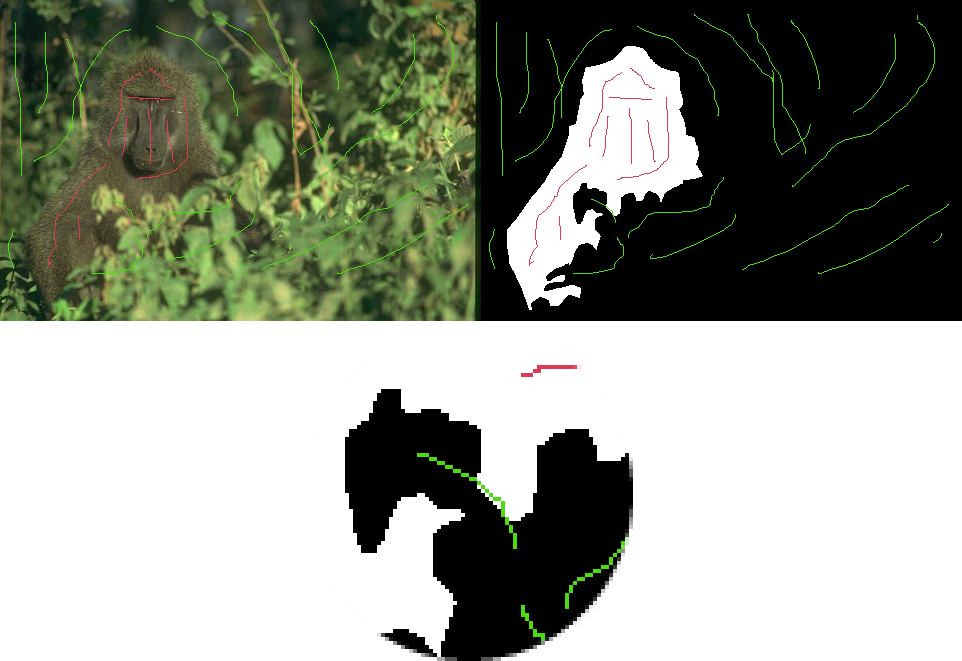
\includegraphics[width=\linewidth]{dilation_error_example}
	\caption{An example of a user error in the annotation process.}
	\label{fig:dilation_error_example}
\end{figure}

\begin{figure}[h]
	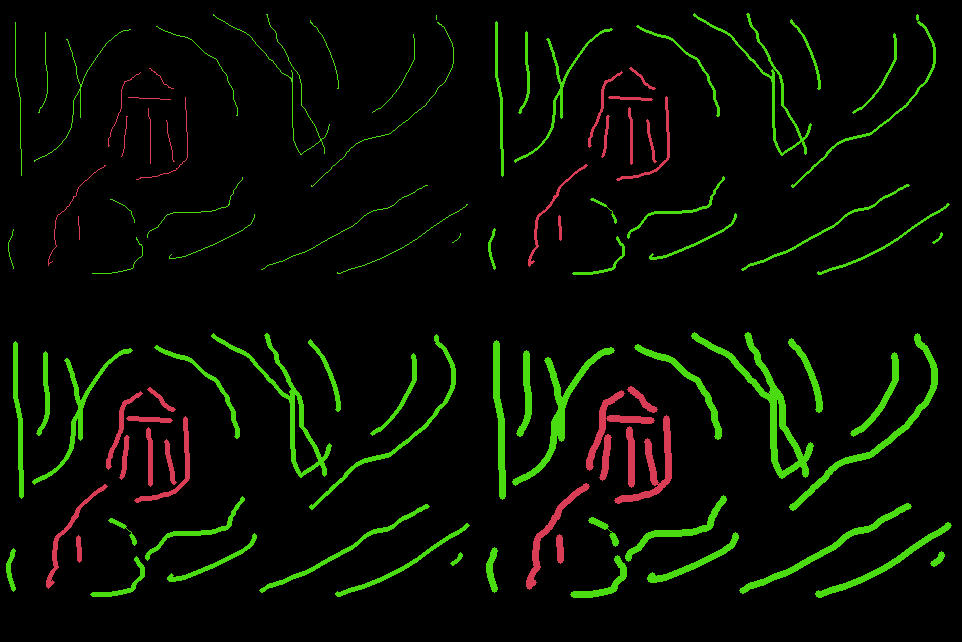
\includegraphics[width=\linewidth]{dilate_example_all}
	\caption{Dilation of radii 1-4 pixels on the label image in figure \ref{fig:dilation_error_example}}
	\label{fig:dilate_example_all}
\end{figure}

The dilation of the label images is the primary independent variable that we're looking at in this study. The dilation was done by setting new pixels as either foreground or background due to their proximity to existing labels. Or put otherwise, all non-zero label pixels would be extended some radius from their center (a value of zero in the label image indicates no label). This dilation is done in a circular fashion, meaning that if the dilation radius is $r$, then all pixels with a Manhattan distance of less than or equal to $r$ will be given the same label.

The fact that dilation is a radius means that the width of a stroke is $2r + 1$. Hence, our upper limit of radius 4 pixel dilation means that strokes have a width of 9 pixels.

In an attempt to avoid introducing \textit{new} errors into the image that the user perhaps wouldn't have made if they were aware of the width of the stroke, we take an approach that depends on ``reading the future'' by glancing at the ground truth and not dilating erroneous labels. For example, if a pixel should be background but the user has marked it with a foreground stroke, then that pixel wouldn't be dilated. However, dilation still occurs for pixels that are correctly placed, but the dilation would spill over into the opposite label. Figure \ref{fig:dilation_error_example} shows an example of a user error here and figure \ref{fig:dilate_example_all} shows the resulting dilation. One can observe the gap that occurs where the background stroke overlaps with the foreground. The gap reduces with higher dilation radii due to dilation still occuring at the closest correctly labeled pixels (and dilating further into the error zone).

Ultimately, this makes little difference as errors tend to be very small. There are, however, a large number of these errors and typically we wouldn't use such an approach to dilate (as it requires knowing the right answer).

\subsection{Segmentation programs}
For the purpose of this study, we used Mark Eramian's implementation of the Boykov graph cut algorithm \cite{boykov_algorithm} as the primary algorithm of interest. This is largely because it is difficult to find ready-to-use algorithms for the purpose of this study and this one is tried and tested in several other studies that have taken place at the University of Saskatchewan \cite{rau}\cite{yuanxia}.

We also used the OneCut algorithm \cite{onecut} as an alternative algorithm to check our results against. We used a modified version \cite{onecutModified} that allowed us to pass our label image in directly in the same manner as the Boykov graph cut algorithm. All images were separately run through both of the segmentation programs. The OneCut algorithm is somewhat of a side consideration as it seems to be extremely sensitive to the number of seeds and thus does not well handle many cases where users simply did not provide very many seeds (noticeable in how it handles points considerably worse than strokes). Figure \ref{fig:onecut_segment_comparison} shows an example of this.

\begin{figure}[h]
	\begin{center}
		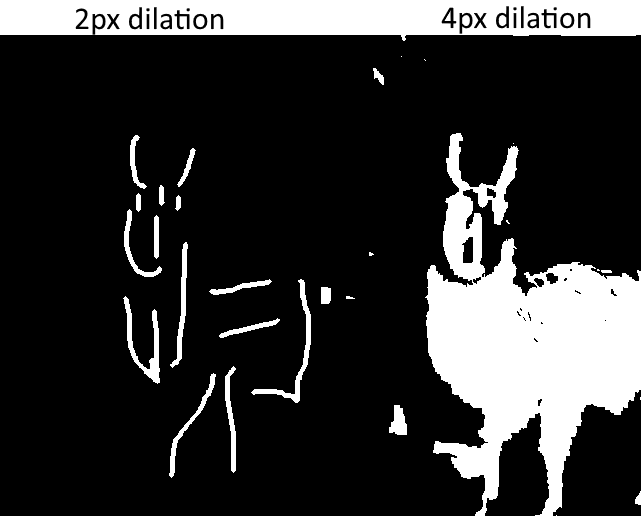
\includegraphics[width=.6\linewidth]{onecut_segment_comparison}
	\end{center}
	\caption{An example of OneCut's poor segmentation when it lacks enough seeds. The image is of a lama and the left case clearly did not segment anything of use -- it merely returned the seeds.}
	\label{fig:onecut_segment_comparison}
\end{figure}

\section{Results}

\subsection{Methods of analysis}
There's two main measures that we looked at in analyzing the segmented results. The accuracy and reproducibility.

We measure accuracy with the Dice Similarity Coefficient (DSC), which is defined as \cite{dsc}:

$$\text{DSC} = \frac{2|X \cap Y|}{|X| + |Y|}$$

Here, $X$ and $Y$ are the sets of pixels in the foregrounds of the image we're analyzing and its associated ground truth. Here, the notation $|X|$ denotes the sum of the binary matrix's elements (ie, how many pixels are in the foreground). The DSC in essence looks at the degree in common that the segmentation has with the ground truth compared to the total number of foreground pixels (thus, it's also considering when the segmentation has too many foreground pixels). Its value will be in between 0 and 1, where 0 implies no match at all and 1 implies a perfect match. Hence, higher values are better.

We measure reproducibility with the Generalized Tanimoto Coefficient (GTC), which is defined as \cite{gtc}:

$$\text{GTC} = \frac{\Sigma_i \left( X_i \wedge Y_i \right)}{\Sigma_i \left( X_i \vee Y_i \right)}$$

Here, $X$ and $Y$ are \textit{all} matrices of binary segmentation of the same image across users (and thus $X_i$ and $Y_i$ are individual matrices, where $X_i \neq Y_i$). Or in other words, we're comparing all pairs of segmented images. What the GTC is essentially saying is that we're looking at what all users got in common (for foreground) and dividing it by what all users had. That tells us how similar the users results were. The ideal segmentation program, after all, would give us similar results (ideally perfect ones) for all reasonable user annotations. We don't want the segmentation program to be vulnerable to extreme inconsistency in results due to exactly where the user places their annotations. The GTC is also a value between 0 and 1, where 0 implies that users all got completely different results and 1 implies they all got the exact same results. Again, higher values are better.

\subsection{Effects on accuracy}
Both the mean and median DSC rose in all of our groups of independent variables when comparing undilated results to 4 pixels of dilation. Figures \ref{fig:steven_mean_dsc} through \ref{fig:yuanxia_median_dsc} show these results. We can observe that mean DSC increases between 0.010 to 0.065 when comparing no dilation to 4 pixels of dilation. There's occasional drops in smaller dilation radii for unknown reasons. It seems to imply some wild inconsistency in how well certain images get segmented (and certainly some are consistently segmented well and others are frequently poorly segmented). Some users simply don't provide as many annotations as others, which is a major cause for some images to segment poorly for them, yet segment well for other users. This only happens for the smaller time pressures in Yuanxia's study, implying that perhaps the placement of annotations by hurried users is simply very poor.

There's some atypical results shown in \ref{fig:yuanxia_median_dsc}, with the median values actually dipping for moderate dilation values, but still ultimately showing an increase between undilated and 4 pixels of dilation. It can be seen from examining the results that sometimes the 1-3 pixel dilation actually has introduced new errors, but it's unclear why this happens (a quirk of the algorithm?).

These results are not normally distributed, so the Friedman test was applied within each independent variable (that is, it was applied to all of the stroke images in Rau's study separately from the point images, etc). This found that all the differences are statistically significant, $p < 0.01$.

\begin{figure}[H]
	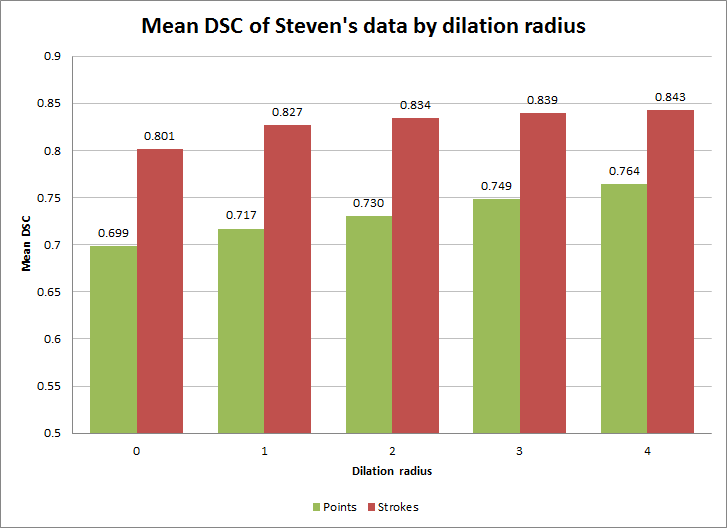
\includegraphics[width=.9\linewidth]{steven_mean_dsc}
	\caption{Mean accuracy in Steven Rau's study.}
	\label{fig:steven_mean_dsc}
\end{figure}

\begin{figure}[H]
	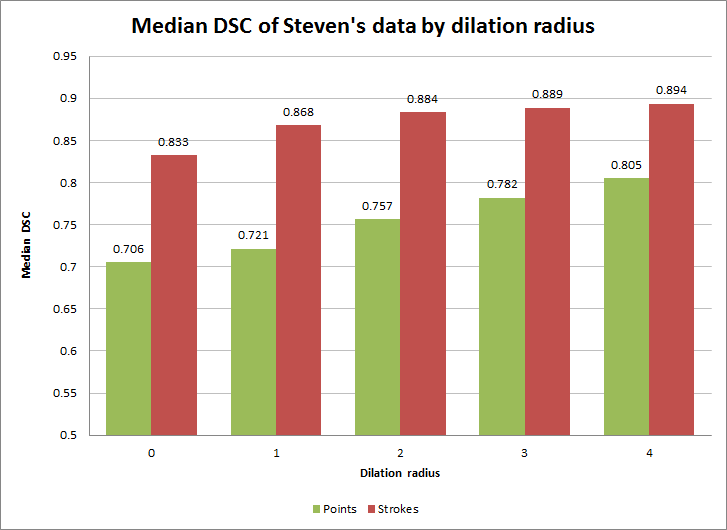
\includegraphics[width=.9\linewidth]{steven_median_dsc}
	\caption{Median accuracy in Steven Rau's study.}
	\label{fig:steven_median_dsc}
\end{figure}

\begin{figure}[H]
	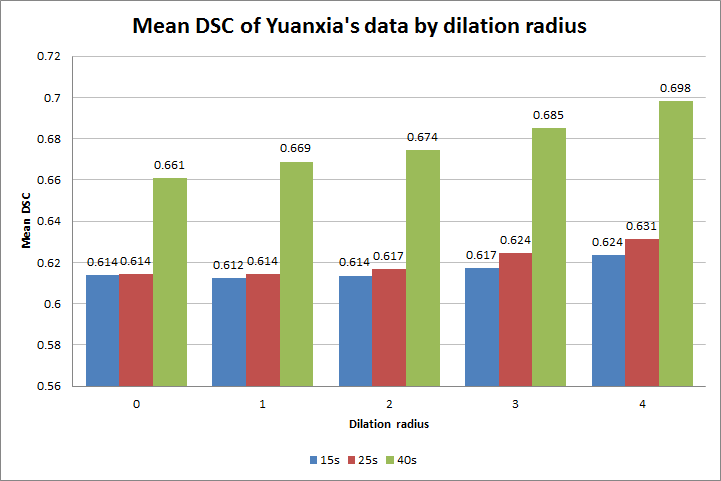
\includegraphics[width=.9\linewidth]{yuanxia_mean_dsc}
	\caption{Mean accuracy in Yuanxia Li's study.}
	\label{fig:yuanxia_mean_dsc}
\end{figure}

\begin{figure}[H]
	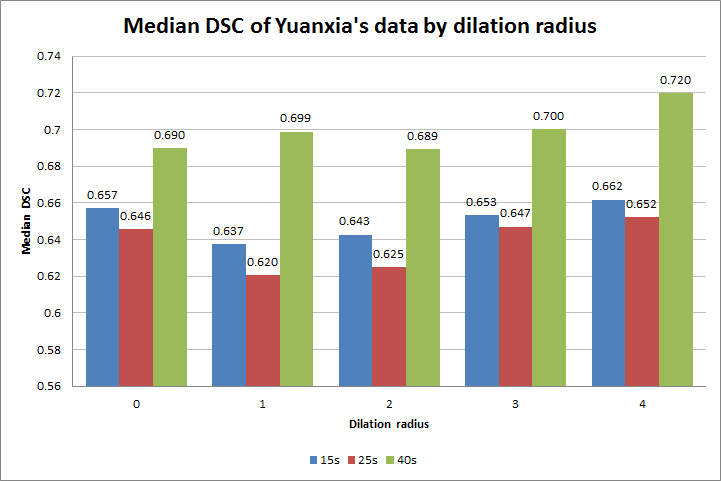
\includegraphics[width=.9\linewidth]{yuanxia_median_dsc}
	\caption{Median accuracy in Yuanxia Li's study.}
	\label{fig:yuanxia_median_dsc}
\end{figure}

\subsection{Effects on reproducibility}
The mean and median GTC has also risen when comparing undilated results to the 4 pixel dilation results. The mean GTC has increased between 0.061 and 0.069 when comparing no dilation versus 4 pixels of dilation. This shows that the increased dilation has made our results more likely to be similar. Figures \ref{fig:steven_mean_gtc} through \ref{fig:yuanxia_median_gtc} show these results.

There's some notable inconsistency in figure \ref{fig:yuanxia_median_gtc}. We note that the GTC of the 15 second time pressure group has actually peaked at smaller dilation radii. The most likely explanation here is simply that rushed-for-time users were very bad at placing annotations and thus obtained some rather wildly varying results.

The Friedman test was also applied to this statistic and found that all the differences are statistically significant, $p < 0.01$.

\begin{figure}[H]
	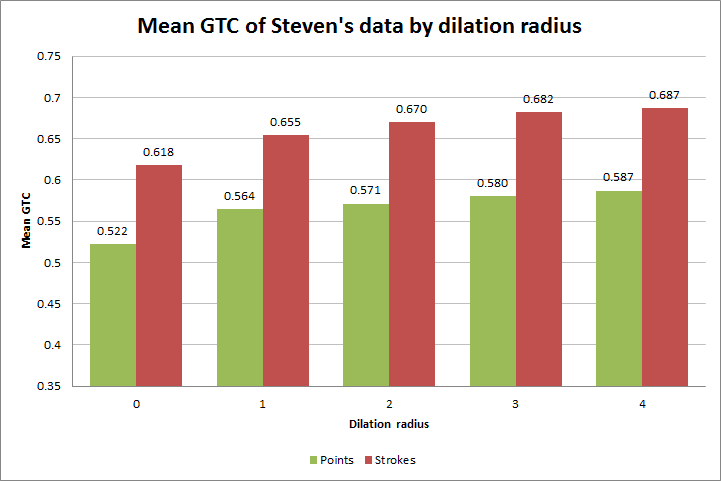
\includegraphics[width=.9\linewidth]{steven_mean_gtc}
	\caption{Mean reproducibility in Steven Rau's study.}
	\label{fig:steven_mean_gtc}
\end{figure}

\begin{figure}[H]
	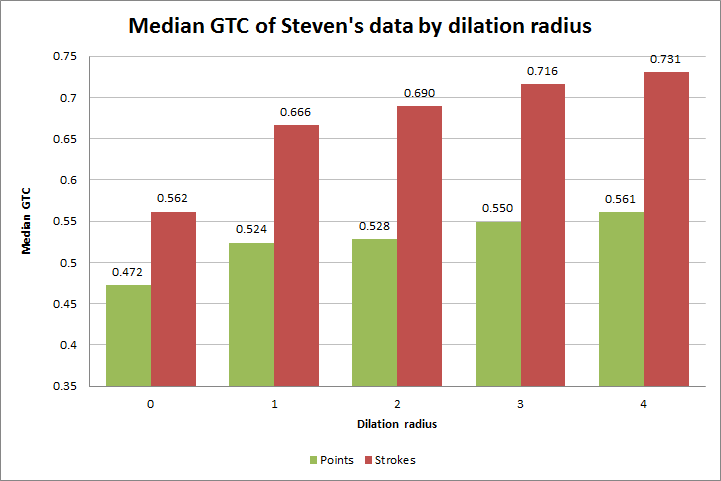
\includegraphics[width=.9\linewidth]{steven_median_gtc}
	\caption{Median reproducibility in Steven Rau's study.}
	\label{fig:steven_median_gtc}
\end{figure}

\begin{figure}[H]
	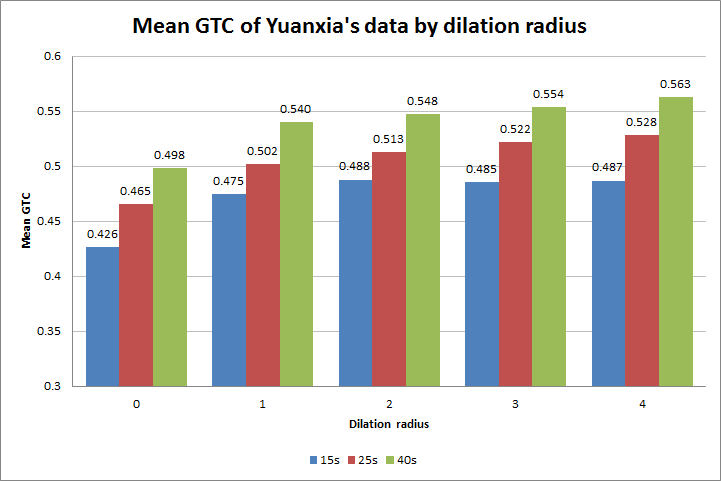
\includegraphics[width=.9\linewidth]{yuanxia_mean_gtc}
	\caption{Mean reproducibility in Yuanxia Li's study.}
	\label{fig:yuanxia_mean_gtc}
\end{figure}

\begin{figure}[H]
	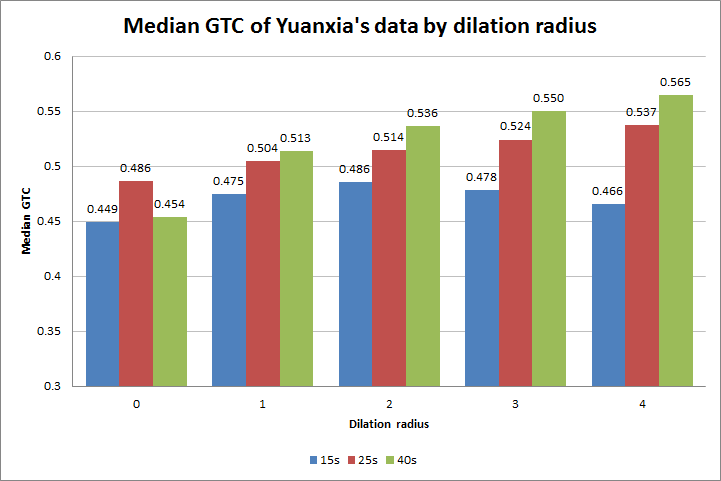
\includegraphics[width=.9\linewidth]{yuanxia_median_gtc}
	\caption{Median reproducibility in Yuanxia Li's study.}
	\label{fig:yuanxia_median_gtc}
\end{figure}

\subsection{Effects with other segmentation algorithms}
We can see in figures \ref{fig:steven_onecut_dsc} and \ref{fig:yuanxia_onecut_dsc} how poorly the OneCut algorithms perform in terms of accuracy. There are some images that they do well at, but many they simply fail to segment in any meaningful way. We can only look so far at this, however, because users were trained on the Boykov graph cut algorithm and thus were working on the expectation that they needed to provide annotations that worked for it. The OneCut algorithm simply seems to need a considerably larger number of seed points to do well. This is evidenced from the massive increases in DSC as the dilation increases. We have to remember, however, that many images aren't actually being segmented (see figure \ref{fig:onecut_segment_comparison}) and thus the dilation naturally will increase the DSC of those images, but without providing any telling results.

The Friedman test showed that the differences in DSC and GTC between the various amounts of dilation (0-4 pixels) were significant with the OneCut algorithm, between all independent variables, $p < 0.01$.

\begin{figure}[H]
	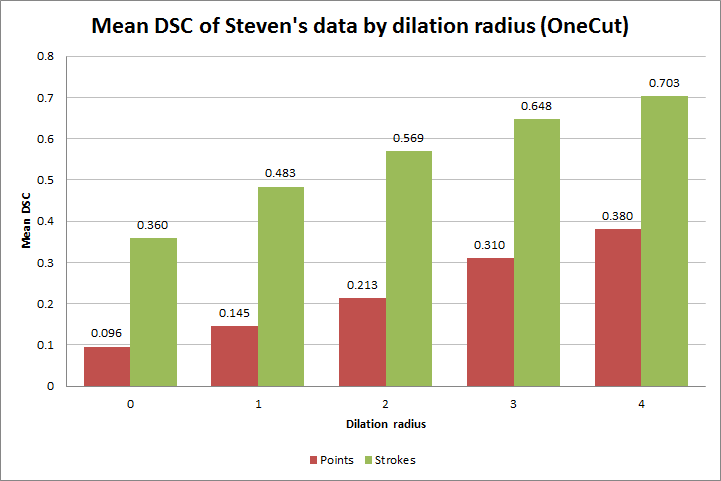
\includegraphics[width=.9\linewidth]{steven_onecut_dsc}
	\caption{Mean OneCut accuracy in Steven Rau's study.}
	\label{fig:steven_onecut_dsc}
\end{figure}

\begin{figure}[H]
	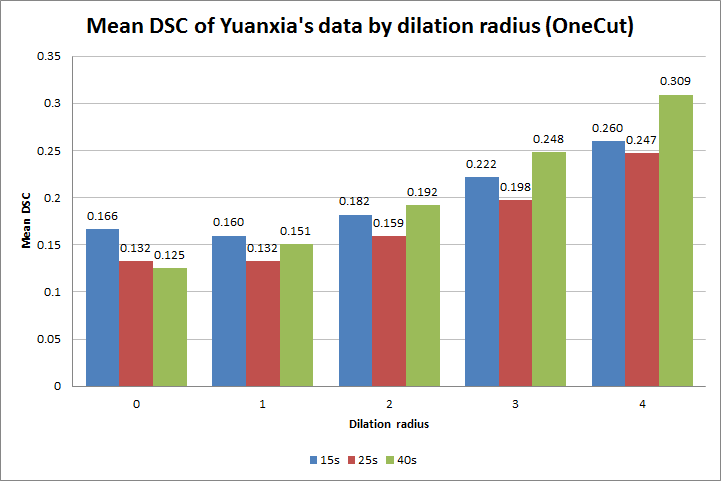
\includegraphics[width=.9\linewidth]{yuanxia_onecut_dsc}
	\caption{Mean OneCut accuracy in Yuanxia Li's study.}
	\label{fig:yuanxia_onecut_dsc}
\end{figure}

The OneCut algorithm's reproducibility seems normal with Rau's data, as we see in figure \ref{fig:steven_onecut_gtc} (if shockingly low -- showing how poorly the algorithm performed with many images). But with Li's data, in figure \ref{fig:yuanxia_onecut_gtc}, we can see that the results were extremely inconsistent from the past trend. Lower time pressures were actually more consistent (higher GTC) and dilation didn't help them so much. It seems that this actually happens because the algorithm occasionally has the very odd behavior of sometimes ``segmenting'' in such a way that everything except the pixels marked as background is considered foreground (and hence resulting in images that are 90\% foreground). This seems to happen less frequently with strokes than points. As well, the higher time pressures have it happening less often (presumably because they have more points). Naturally having almost all the image being considered foreground would be considered very consistent (if flat out wrong). This is also a good example of why we don't want to look at the GTC in a vacuum, as we can have results that are consistently wrong scoring a high GTC.

The Friedman test showed that all of these results \textit{except} for that of Li's 40 second group were significant, $p < 0.01$.

\begin{figure}[H]
	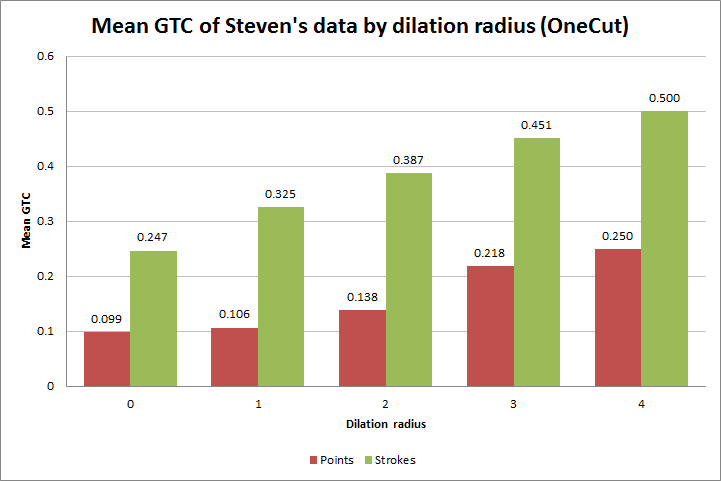
\includegraphics[width=.9\linewidth]{steven_onecut_gtc}
	\caption{Mean OneCut reproducibility in Steven Rau's study.}
	\label{fig:steven_onecut_gtc}
\end{figure}

\begin{figure}[H]
	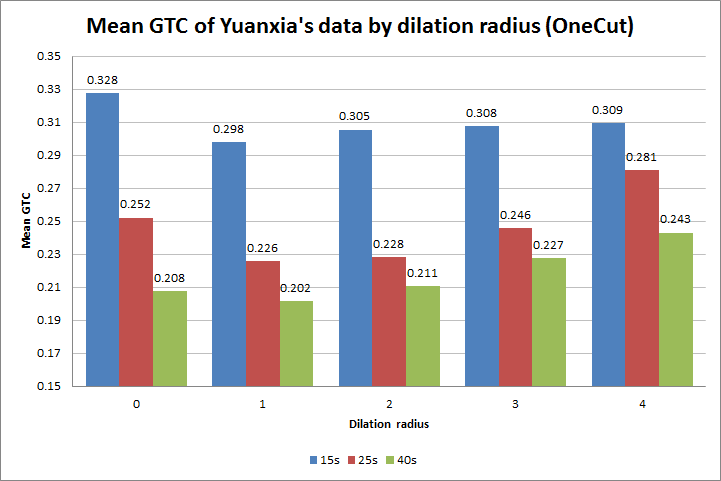
\includegraphics[width=.9\linewidth]{yuanxia_onecut_gtc}
	\caption{Mean OneCut reproducibility in Yuanxia Li's study.}
	\label{fig:yuanxia_onecut_gtc}
\end{figure}

\section{Conclusion and discussion}
The results are not always completely consistent, but in general, we can conclude that the difference between no dilation and 4 pixels of dilation is a statistically significant increase in accuracy and reproducibility (certainly at least with the Boykov algorithm). In general, we get better results with dilation if we allow users time to place annotations, as we observe that low time pressures sometimes get more finnicky results. It was known from Rau's study that strokes perform better than points \cite{rau}, which was surely due to the larger number of seeds. But we can also see that we can go further, still.

The results can be highly variable by user, however. Some users simply do not provide enough annotations for segmentation to work well. Dilation can improve this, but can only do so much. Users simply spending more time and effort to provide a larger set of annotations makes a considerable difference both with and without the dilation. Arguably software that utilizes semi-automatic image segmentation in this technique should not only use thicker strokes, but also ensure that users are aware of the impact of simply adding more annotations.

One notable question is if we might get different results if users were aware of the larger ``pen size''. Might they make fewer errors and redundancies? This would also avoid the need for our dilation algorithm to utilize a non-traditional approach in trying to avoid introducing new errors. There's the worry that this approach could create unrealistic results.

There was some cases where moderate amounts of dilation actually introduced worse results (see figure \ref{fig:yuanxia_median_dsc}). There was still an increase for radius 4 pixel dilation, however. It's unclear why the algorithm acts this way. The segmentation ends up being fairly different, but there's no obvious explanations for this and it's something that would need further study. This only occurred in the results from Li's study, so perhaps the time pressures are related to this. An analysis could be done on if these odd dilation results correlate with user errors or the like, since the time pressure introduced more errors.

The OneCut algorithm that we tested proved interesting. In general, it should probably be regarded as little more than a side consideration in this study. There's the big issue that users were not trained with this algorithm and thus did not realize that it is much more sensitive to how much information is provided. As well, it just plain works very poorly on undilated label images. It was clearly not created with so few seeds in mind and the Rau and Li studies were not designed with that requirement. Hence, the provided user data is insufficient to well test it, especially when we have so many cases of no segmentation occuring, which essentially ends up statistically drowning out relevant results. However, we can at least conclude that the OneCut algorithm is extremely sensitive to the amount of annotations and thus recommend that its users provide many, thick strokes if they wish to get meaningful results.

The fact that semi-automatic image segmentation algorithms seem sensitive the quantity of seed points (which is really what dilating the strokes is doing) also serves to partially explain the results of strokes versus points. Stroke annotations naturally provide more seed points than point annotations, as dilation does. That said, strokes are much more efficient than points because they provide more \textit{useful} annotations (due to greater range of area). And as we've shown, thicker strokes perform better still.

This does also mean that in comparing the results of studies that utilize a seed-based approach for semi-automatic image segmentation, we must consider the width of the strokes used. As well, the width should also be consistent within the study in order to have truly comparable results.

The code and data for this study are available online at \url{https://github.com/KatrinaHoffert/stroke-radius-segmentation} \cite{repo}.

\bibliographystyle{./IEEEtran/bibtex/IEEEtran}
\bibliography{bibliography}

\end{document}